\chapter{实验结果与分析}
\label{cha:experiments}

本章按照第四章定义的实验协议，分析 YOLO 双目标检测模型在边缘设备端的表现。实验并不只报告一个离线精度数值，而是先用官方基线、YOLOv8n 场景化训练结果和板端 FP16/OM 结果建立参照系，再分别考察全量验证集检测能力、分类别语义、置信度阈值、NMS 参数、应用层后处理、代表性视频片段和分段计时口径。这样安排后，板端结果可以和训练阶段能力、部署规则以及运行时状态放在同一证据链中解释。

\section{实验设置与评价范围}

本文实验使用同一轻量 YOLO 双目标检测模型，类别为 \textit{person} 与 \textit{ebike}。图像验证集包含 720 张电梯轿厢图像，评价指标包括 precision、recall、F1、mAP@0.5、分类别指标和板端运行状态。板端推理使用搭载华为海思 Hi3516DV500 视觉 SoC 的 HongOU PI 开发板完成，模型以 OM 离线模型形式运行，后处理包含置信度筛选和 NMS。

表 \ref{tab:board_platform_specs} 给出了本文实验使用的板端平台与部署工具链。该信息用于限定本文所有板端指标的硬件和运行口径，后续检测指标、参数敏感性、视频稳定性和分段计时结果均基于同一类部署环境获得。

\begin{table}[htbp]
    \centering
    \caption{板端实验平台与部署工具链}
    \label{tab:board_platform_specs}
    \begin{tabular}{p{3.0cm} p{7.6cm}}
        \toprule
        项目 & 配置 \\
        \midrule
        开发板 & HongOU PI（Hi3516DV500） \\
        平台定位 & 国产边缘 AI 视觉 SoC 开发平台 \\
        核心 SoC & 华为海思 Hi3516DV500 视觉 SoC \\
        CPU & 双核 ARM Cortex-A55 @ 850 MHz \\
        DDR & 2 GB DDR4 \\
        eMMC & 8 GB \\
        NPU & 2 TOPS INT8 NN 算力 \\
        模型格式 & OM 离线模型 \\
        部署工具链 & ATC / CANN / SVP\_NPU \\
        交叉编译目标 & AArch64 GNU/glibc 工具链 \\
        \bottomrule
    \end{tabular}
\end{table}

图 \ref{fig:board_photo} 展示了本文实验使用的 HongOU PI（Hi3516DV500）开发板实物。该开发板体积紧凑，适合嵌入电梯控制柜或轿厢顶部安装，板载接口支持摄像头视频输入和网络数据传输。

\begin{figure}[htbp]
    \centering
    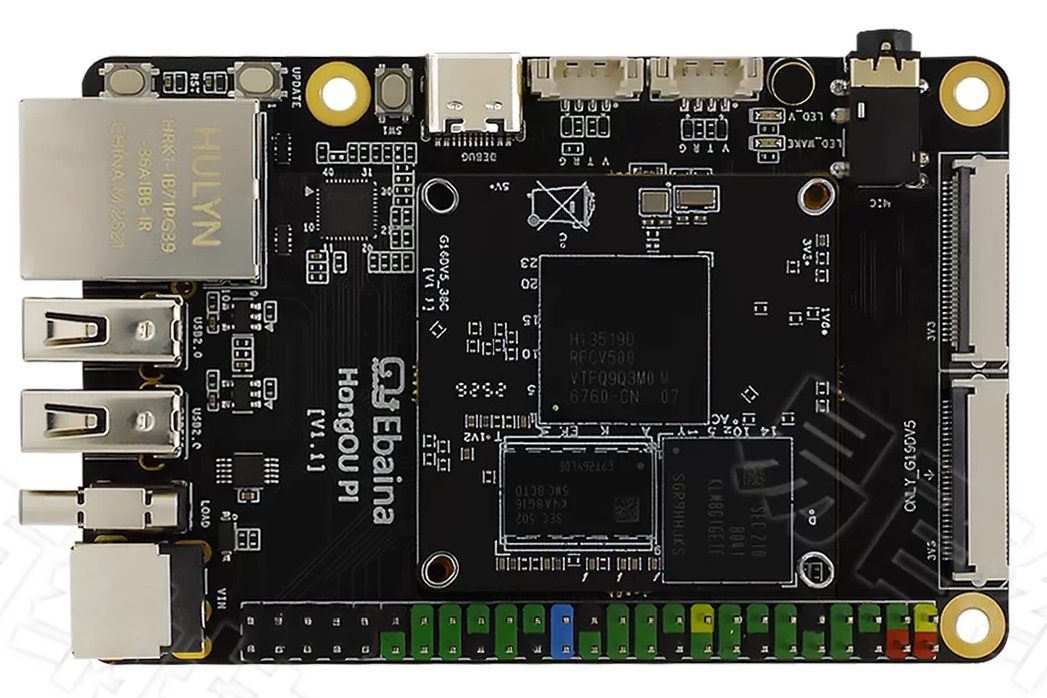
\includegraphics[width=0.55\textwidth]{image/fig_board_photo.png}
    \caption{HongOU PI（Hi3516DV500）开发板实物}
    \label{fig:board_photo}
\end{figure}

实验前先确认板端验证环境、模型文件、应用程序和数据集均处于就绪状态。全量验证集已完成板端实测，阈值敏感性分析采用既有板端检测输出进行后验筛选重算；NMS 和后处理消融采用同一板端 campaign 协议，保证只有一个参数变化；分段计时实验则使用新增计时埋点对小样本 batch 图像验证和代表性视频片段进行补充复查。

阈值后验重算的依据是板端检测输出中保留了每个候选框的类别、置信度和坐标，同时每张图像具有对应真实标注。因此，在原始候选阈值低于待分析阈值的前提下，可以通过重新筛选候选框并按 IoU@0.5 匹配真实框，得到不同置信度阈值下的 precision、recall 和 F1。该做法不改变模型推理结果，只改变结果解释阈值，适合用于分析安全输出对阈值选择的敏感程度。

本章评价问题与证据形式保持一一对应。RQ1 使用 720 张图像完整验证总体指标回答板端完整验证是否可执行且具备检测能力；RQ2 使用分类别 TP、FP、FN、recall 和 mAP@0.5 检查两类目标是否保持正确语义；RQ3 使用 0.20--0.40 置信度阈值后验重算分析安全输出稳定性；RQ4 和 RQ5 分别使用固定 score 后改变 NMS 阈值、改变电动车清理策略的板端 campaign；RQ6 使用代表性视频片段和平滑窗口对比观察连续输出；RQ7 使用 50 张图像 batch 复查与连续视频分段计时解释运行时指标。这样的组织方式用于保证每个实验结论都能追溯到具体数据类型，避免把不同口径的指标混为一谈。

\section{板端检测能力验证}

\subsection{板端完整验证集结果}

表 \ref{tab:board_overall_results} 给出了 720 张图像验证集上的总体结果。所有样本均在板端完成处理，成功处理样本数为 720，失败样本数为 0。总体 precision 为 0.901，recall 为 0.923，F1 为 0.912，mAP@0.5 为 0.910。板端 batch 图像验证链路端到端平均单图处理耗时约为 1119.510 ms。

\begin{table}[htbp]
    \centering
    \caption{边缘设备端总体检测结果}
    \label{tab:board_overall_results}
    \begin{tabular}{l c}
        \toprule
        指标 & 数值 \\
        \midrule
        验证图像数 & 720 \\
        成功样本数 & 720 \\
        失败样本数 & 0 \\
        precision & 0.901 \\
        recall & 0.923 \\
        F1 & 0.912 \\
        mAP@0.5 & 0.910 \\
        batch 端到端单图处理耗时/ms & 1119.510 \\
        \bottomrule
    \end{tabular}
\end{table}

这组数据至少说明两点。第一，YOLOv8n 场景化训练模型经过 ONNX 导出、ATC 编译和 OM 部署后，能够在边缘设备上跑完 720 张验证图像。第二，板端输出可以继续计算 precision、recall、F1 和 mAP@0.5，说明后续分类别分析、阈值扫描和运行时拆解有共同的数据基础。

表 \ref{tab:board_overall_results} 中的 1119.510 ms 是 batch 图像验证链路的端到端单图处理耗时，包含图像输入、媒体链路、预处理、模型执行、后处理和结果写出等环节。它描述的是验证路径整体成本，不能等同于 OM 模型执行阶段耗时，也不能直接代表连续视频链路的帧间处理时间。后续分段计时实验会专门拆开这一差异。

\subsection{训练阶段与板端同集对比}

为了避免将板端指标孤立理解，本文把第五章结果放入同一任务证据链中解释。证据链包括官方 YOLOv8n COCO-person 基线、基于 RTX 3090 GPU 完成训练的 YOLOv8n 场景化模型，以及 Hi3516DV500 板端 FP16/OM 完整验证结果。前者用于说明通用预训练模型直接迁移到电梯俯视场景时的不足，中间结果作为训练阶段能力参照，板端结果则用于衡量部署后检测能力是否被保留。三者共同回答的问题不是“本文指标在所有公开数据集上排名如何”，而是在同一电梯验证集和同一安全任务背景下，模型从通用基线、场景训练到板端部署的效果变化是否具有解释性。

表 \ref{tab:stage_comparison_evidence} 给出了三类证据的来源和可比性边界。官方 YOLOv8n 基线采用已修正的 COCO-person 逐图 IoU 匹配评估口径，precision 为 0.743，recall 为 0.728，F1 为 0.736。该基线只评价 \textit{person} 类别，不能与双类别 mAP@0.5 直接等价，但可以作为通用 COCO person 能力在电梯俯视场景中的低基线。YOLOv8n 场景化训练模型第 100 个 epoch 的 precision 为 0.976，recall 为 0.965，mAP@0.5 为 0.988；板端 FP16/OM 完整验证的 precision 为 0.901，recall 为 0.923，F1 为 0.912，mAP@0.5 为 0.910。

\begin{table}[htbp]
    \centering
    \caption{训练阶段与板端同集对比证据}
    \label{tab:stage_comparison_evidence}
    \begingroup
    \zihao{5}
    \setlength{\tabcolsep}{4pt}
    \renewcommand{\arraystretch}{1.25}
    \begin{tabular}{@{}p{2.4cm}p{3.0cm}p{3.2cm}p{4.2cm}@{}}
        \toprule
        阶段 & 环境与格式 & 核心指标 & 可比性说明 \\
        \midrule
        COCO-person 基线 & \makecell[l]{官方 YOLOv8n\\逐图评估} & \makecell[l]{P=0.743\\R=0.728\\F1=0.736} & 只评价 person 类别，用于说明通用模型不足 \\
        YOLOv8n 场景化训练 & \makecell[l]{PyTorch/Ultralytics\\RTX 3090 GPU} & \makecell[l]{P=0.976\\R=0.965\\mAP@0.5=0.988} & 训练阶段双目标检测参照 \\
        Hi3516DV500 板端 & \makecell[l]{OM 离线模型\\FP16/板端应用} & \makecell[l]{P=0.901\\R=0.923\\F1=0.912\\mAP@0.5=0.910} & 部署后完整 720 张验证集实测 \\
        \bottomrule
    \end{tabular}
    \endgroup
\end{table}

图 \ref{fig:chap05_stage_comparison} 展示了阶段间指标关系。左侧使用 precision、recall 和 F1 比较三类证据，可以看到 YOLOv8n 场景化训练模型相比官方 COCO-person 基线有明显提升，说明电梯轿厢中的俯视视角、遮挡和目标形态差异需要场景化训练支撑。右侧比较训练阶段验证结果与板端 FP16/OM 结果的 mAP@0.5，板端结果相比训练阶段下降约 0.078。这一差异来自模型导出、OM 编译、板端预处理、输出解码和后处理链路的共同影响；不过板端 mAP@0.5 仍达到 0.910，主要检测能力在部署后得到了保留。

\begin{figure}[htbp]
    \centering
    
\includegraphics[width=\textwidth]{image/generated/fig_chap05_stage_comparison.pdf}
    \caption{官方基线、YOLOv8n 训练阶段与板端 FP16/OM 结果对比}
    \label{fig:chap05_stage_comparison}
\end{figure}

后续阈值敏感性、NMS 敏感性、后处理消融和分段计时实验，并不是对一个孤立板端数值的简单补充，而是在“训练阶段能力已经建立、板端部署后存在可量化回退”的前提下，继续解释部署链路中哪些因素会影响最终安全输出。

\subsection{分类别输出分析}

表 \ref{tab:board_class_results} 给出了 \textit{person} 与 \textit{ebike} 两类目标的检测结果。电动车类别的 mAP@0.5 为 0.952，召回率为 0.961，高于行人类别的 0.869 和 0.888。这说明在当前验证集上，模型对电动车目标具有较强识别能力，而行人类别受到遮挡、截断和多人重叠等因素影响更明显。

\begin{table}[htbp]
    \centering
    \caption{边缘设备端分类别检测结果}
    \label{tab:board_class_results}
    \begin{tabular}{lrrrrrrr}
        \toprule
        类别 & GT & Pred & TP & FP & FN & recall & mAP@0.5 \\
        \midrule
        person & 776 & 794 & 689 & 105 & 87 & 0.888 & 0.869 \\
        ebike & 720 & 739 & 692 & 47 & 28 & 0.961 & 0.952 \\
        \bottomrule
    \end{tabular}
\end{table}

图 \ref{fig:chap05_detection_metrics} 对总体指标和分类别指标进行了可视化。整体四项指标均处于 0.90 左右，说明板端输出具备基本检测能力；分类别结果中，电动车类别的召回率和 mAP@0.5 均高于行人类别，符合电动车结构特征更清晰、行人更容易受近景截断和多人重叠影响的场景观察。

\begin{figure}[htbp]
    \centering
    
\includegraphics[width=\textwidth]{image/generated/fig_chap05_detection_metrics.pdf}
    \caption{边缘设备端总体指标与分类别指标}
    \label{fig:chap05_detection_metrics}
\end{figure}

为补充分类别指标的直观解释，图 \ref{fig:chap05_board_val_examples} 给出了从 720 张完整验证集板端输出中按固定规则抽取的检测示例。图中底图来自验证集原图，检测框和置信度来自 HongOU PI（Hi3516DV500）开发板生成的检测记录，并按板端记录的帧尺寸恢复到图像坐标。示例筛选条件为样本运行成功、同时包含 \textit{person} 与 \textit{ebike}、两类均产生 TP 且无 FP/FN；在满足上述条件的样本中，优先选择检测置信度较高、目标边界不贴边且可视化较清晰的样本。该图用于展示板端输出形态，完整性能判断仍以表 \ref{tab:board_class_results} 和图 \ref{fig:chap05_detection_metrics} 的全量统计为准。

\begin{figure}[htbp]
    \centering
    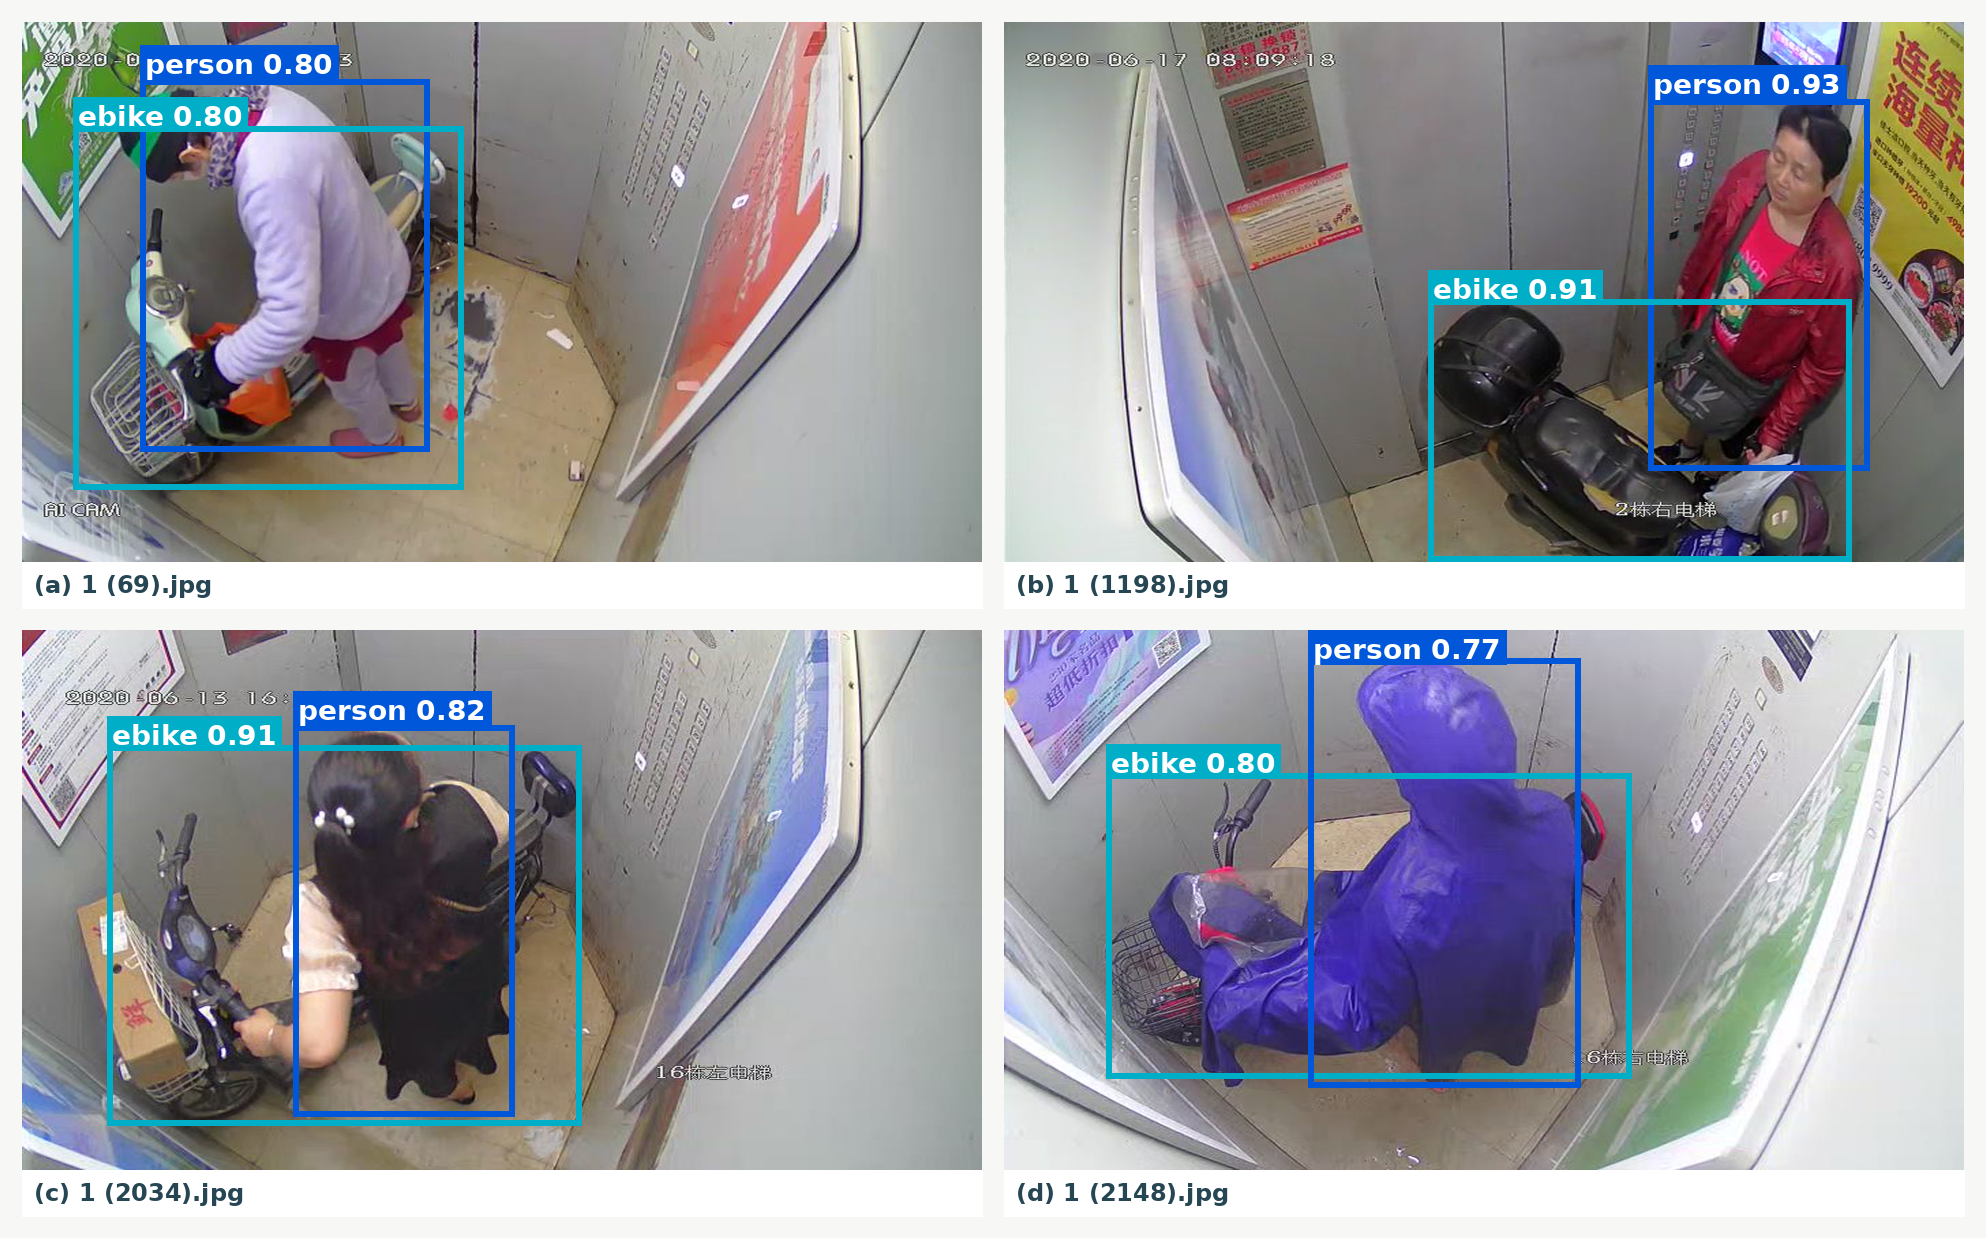
\includegraphics[width=\textwidth]{image/generated/fig_chap05_board_val_examples.png}
    \caption{Hi3516DV500 板端检测输出示例}
    \label{fig:chap05_board_val_examples}
\end{figure}

从部署行为对照的角度看，分类别统计还可以反向验证类别契约是否成立。如果类别顺序在导出或板端解析过程中发生错位，\textit{person} 与 \textit{ebike} 的 TP、FP、FN 分布会出现明显异常，难以呈现当前这种与场景经验一致的分类别结果。因此，分类别指标不仅用于衡量检测性能，也是部署语义检查的一部分。

\section{部署参数敏感性分析}

\subsection{阈值敏感性分析}

为分析置信度阈值对安全输出的影响，本文在既有板端检测输出基础上进行后验筛选重算。由于原始板端运行使用的候选阈值低于本节扫描阈值，本文可以在不重新推理的条件下，分别保留置信度不低于 0.20、0.25、0.30、0.35 和 0.40 的检测框，并按 IoU@0.5 重新统计 precision、recall 和 F1。表 \ref{tab:threshold_sensitivity_results} 给出了结果。

\begin{table}[htbp]
    \centering
    \caption{置信度阈值敏感性后验重算结果}
    \label{tab:threshold_sensitivity_results}
    \begin{tabular}{cccccc}
        \toprule
        conf & precision & recall & F1 & ebike recall & person recall \\
        \midrule
        0.20 & 0.911 & 0.919 & 0.915 & 0.957 & 0.884 \\
        0.25 & 0.921 & 0.916 & 0.919 & 0.957 & 0.878 \\
        0.30 & 0.925 & 0.912 & 0.919 & 0.956 & 0.872 \\
        0.35 & 0.935 & 0.909 & 0.922 & 0.956 & 0.866 \\
        0.40 & 0.942 & 0.903 & 0.922 & 0.953 & 0.857 \\
        \bottomrule
    \end{tabular}
\end{table}

随着置信度阈值从 0.20 提高到 0.40，总体 precision 从 0.911 提升到 0.942，recall 从 0.919 下降到 0.903，F1 保持在 0.915--0.922 区间。电动车召回率在五个阈值下保持在 0.953 以上，说明在当前验证集和板端输出条件下，电动车检测对这一阈值区间不太敏感。行人召回率随阈值提高从 0.884 降至 0.857，说明行人类别中存在更多接近阈值边界的候选框。

图 \ref{fig:chap05_threshold_sensitivity} 展示了各指标随阈值变化的趋势。precision 随阈值提高而上升，recall 缓慢下降，F1 保持相对平稳；分类别召回率中，\textit{ebike} 曲线较平，\textit{person} 曲线下降更明显。阈值选择不能只依据总体 F1，还需要考虑不同类别在安全任务中的风险权重。

\begin{figure}[htbp]
    \centering
    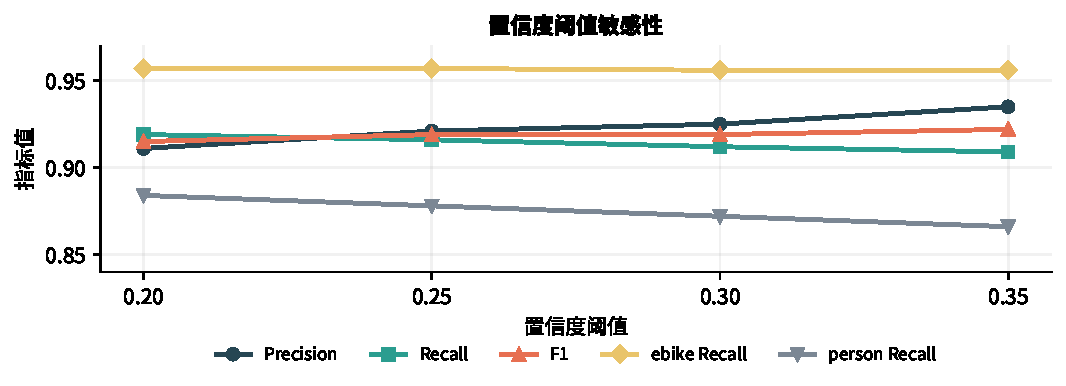
\includegraphics[width=\textwidth]{image/generated/fig_chap05_threshold_sensitivity.pdf}
    \caption{置信度阈值敏感性曲线}
    \label{fig:chap05_threshold_sensitivity}
\end{figure}

阈值敏感性后验重算并不等同于重新训练模型，也不改变板端推理输出。它的作用是分析同一批板端输出在不同安全阈值下的波动情况，因此可以增强本文关于当前验证集内阈值行为的证据链。

\subsection{NMS 参数敏感性}

NMS 参数敏感性实验关注的是重叠候选框如何被保留。实验固定模型、验证集、置信度阈值和后处理策略，只改变 NMS 阈值，取值为 0.35、0.45 和 0.55。阈值较低时，相邻候选框会被更强地抑制，重复框可能减少，但遮挡区域也更容易漏检；阈值较高时，局部目标的候选框保留更多，误报和重复框也可能随之增加。

这组实验不同于阈值后验重算，需要重新运行板端推理，因为 NMS 已经在板端应用层改变最终输出。三组实验使用同一 OM 模型、同一板端二进制和同一验证集切分，均处理 720 张图像，失败样本数为 0。

结果显示，NMS 从 0.35 提高到 0.55 时，预测框总数从 1526 增至 1542，FP 从 146 增至 160，FN 从 116 降至 114。行人类别 F1 在三组设置下均为 0.878，变化很小；电动车 F1 从 0.952 降至 0.944，而电动车召回率从 0.960 小幅升至 0.963。可以看出，提高 NMS 阈值会多保留一些电动车候选框，漏检略少，但误报也增加，因此 F1 略有下降。

\begin{figure}[htbp]
    \centering
    
\includegraphics[width=\textwidth]{image/generated/fig_chap05_nms_sensitivity.pdf}
    \caption{NMS 参数敏感性结果}
    \label{fig:chap05_nms_sensitivity}
\end{figure}

从安全场景角度看，NMS=0.45 是较平衡的设置：其 mAP@0.5 为 0.910，整体 FP/FN 分别为 152 和 115，与 0.55 的 mAP@0.5 基本相当，但误报更少；与 0.35 相比，0.45 保留了略多候选框并取得更高 mAP@0.5。本文采用的 NMS 设置并不是孤立参数，而是在召回、误报和重复框保留之间取得折中。

\subsection{后处理策略消融}

应用层后处理消融用于回答一个容易混淆的问题：板端输出变化究竟来自模型权重，还是来自模型之后的候选框清理逻辑。后处理消融中，电动车误检清理策略被显式暴露为 full、safe 和 off 三种模式。其中，full 表示完整启用误检清理，safe 表示只启用较保守的重复框和明显条带清理，off 表示关闭电动车类别特定清理。默认 auto 模式保持当前板端行为，即 batch 评价路径保留更原始的 safe 输出，视频 file 路径使用更面向展示的 full 输出。

该消融不是训练消融，也不表示本文提出了新的检测网络结构。它的作用是把板端应用层规则从“隐含工程细节”转化为可以复查的部署模块。三组实验均完成 720 张验证图像，失败样本数为 0，产物分别对应 cleanup\_full、cleanup\_safe 和 cleanup\_off campaign。

full 策略将电动车 FP 从 safe 的 47 降至 38，但电动车 FN 从 28 增至 169，电动车 recall 从 0.961 降至 0.765，F1 从 0.949 降至 0.842。也就是说，完整清理策略确实减少了部分电动车误报，但代价是过度抑制真实电动车候选框。相比之下，safe 策略保留较高电动车召回率；off 策略进一步将电动车 recall 提高到 0.963，但 FP 增至 55，F1 降至 0.944。

\begin{figure}[htbp]
    \centering
    
\includegraphics[width=\textwidth]{image/generated/fig_chap05_postprocess_ablation.pdf}
    \caption{后处理策略消融结果}
    \label{fig:chap05_postprocess_ablation}
\end{figure}

这一组结果提醒本文不能只讨论模型权重，应用层后处理策略同样会改变最终输出。对于图像验证链路，safe 策略在误报控制和召回保持之间更平衡，因此更适合作为板端 batch 分析的默认口径；full 策略可用于展示链路中的强清理，但不宜直接作为图像级检测指标的默认设置。正文评价以完整验证集统计为主，定性样例和视频片段用于补充说明输出形态与连续性。

\section{运行时评价}

\subsection{视频稳定性观察}

除图像验证集外，本文还使用代表性视频片段观察连续场景下的输出波动。机器侧统计显示，在一个约 14.58 s、437 帧的代表性片段中，系统能够记录原始检测输出、筛选后输出、分段计时和运行资源信息。视频片段评价采用检测保持率、闪烁窗口、连续无输出片段和分段计时等机器侧指标，用于观察连续帧中的检测保持、闪烁、漏检现象和运行时状态。

视频稳定性实验固定模型、score 和 NMS，只改变平滑窗口，重点比较窗口 1 与窗口 5。前者接近无平滑或最小平滑，能够暴露单帧检测分数波动；后者代表默认连续输出策略，更接近真实展示链路。两组实验均处理 437 帧，产物分别为 video\_smooth1 和 video\_smooth5。

从逐帧输出看，两组实验的检测保持率均为 0.982，均出现 3 个 person\_flash 闪烁窗口，闪烁帧数均为 5，连续无输出片段数均为 2，最长无输出片段为 5 帧。窗口 1 与窗口 5 在该代表性片段上的输出统计基本一致，说明当前片段中主要波动不是简单通过增大平滑窗口即可消除的单帧噪声。两组视频路径的单帧处理耗时均值分别为 11.811 ms 和 11.951 ms，模型执行耗时均值分别为 8.359 ms 和 8.365 ms，均低于 30 fps 对应的 33.3 ms 帧间隔。

\begin{figure}[htbp]
    \centering
    
\includegraphics[width=\textwidth]{image/generated/fig_chap05_video_stability.pdf}
    \caption{代表性视频片段稳定性结果}
    \label{fig:chap05_video_stability}
\end{figure}

视频片段分析表明，安全视觉系统的最终输出不仅取决于单帧检测框，还取决于后处理策略和连续帧稳定性。即使图像级指标较高，若连续视频中目标框频繁出现和消失，仍会影响预警体验。因此，本文将视频分析作为图像验证集的补充。本节的“检测保持率”和“连续无输出片段”描述连续输出状态，图像级检测精度仍由 720 张验证集结果承担。

\subsection{分段计时分析}

为避免把 batch 图像验证链路端到端耗时误解为 OM 模型执行阶段耗时，本文补充了板端分段计时实验。该实验在应用程序中记录单帧处理、模型执行、预处理、后处理和渲染等分段字段。其中，端到端字段表示 batch 图像验证链路单图耗时，单帧处理字段表示核心处理路径耗时，模型执行字段表示包围 OM/NPU 模型执行调用的工程计时。

表 \ref{tab:timing_breakdown_results} 给出了本轮分段计时结果。50 张图像 batch 复查中，端到端耗时均值为 1123.300 ms，与 720 张完整验证集中的 1119.510 ms 处于同一数量级；但同一实验中的单帧处理耗时均值为 21.459 ms，模型执行耗时均值为 8.208 ms。代表性视频片段中，单帧处理耗时均值为 11.870 ms，模型执行耗时均值为 8.407 ms。

\begin{table}[htbp]
    \centering
    \caption{板端分段计时结果}
    \label{tab:timing_breakdown_results}
    \begin{tabular}{lrrrr}
        \toprule
        运行模式 & 样本规模 & 端到端耗时 & 单帧处理耗时 & 模型执行耗时 \\
        \midrule
        batch 图像验证 & 50 张图像 & 1123.300 & 21.459 & 8.208 \\
        连续视频处理 & 437 帧 & -- & 11.870 & 8.407 \\
        \bottomrule
    \end{tabular}
\end{table}

图 \ref{fig:chap05_timing_breakdown} 使用对数坐标展示上述差异，图中虚线表示 30 fps 视频约 33.3 ms 的帧间隔。可以看到，batch 端到端耗时与单帧核心处理、模型执行阶段不在同一数量级。这说明 1119.510 ms 指标主要用于描述 batch 图像验证路径的端到端成本，而不应解释为模型执行阶段耗时。代表性视频路径下的单帧核心处理耗时低于 33.3 ms，说明该按源帧节奏回放条件下的处理计时与连续帧输入节奏相容；这一结论属于运行时分段证据，用于补充图像验证集指标。

\begin{figure}[htbp]
    \centering
    
\includegraphics[width=\textwidth]{image/generated/fig_chap05_timing_breakdown.pdf}
    \caption{板端分段计时结果对比（对数坐标）}
    \label{fig:chap05_timing_breakdown}
\end{figure}

分段计时结果的适用范围由运行模式决定。50 张图像 batch 复查用于解释运行时口径，并与 720 张完整验证集检测指标形成互补；代表性视频片段说明连续处理路径和运行时耗时；模型执行耗时则是当前模型、二进制、阈值和板端环境下的工程观测值，用于佐证本文关于部署行为是否对齐的分析。

\section{综合讨论}

\subsection{部署一致性综合分析}

把训练阶段和板端结果放在一起看，官方 COCO-person 基线不足以支撑电梯俯视场景检测，场景化训练后的 YOLOv8n 明显提高了同集检测能力。模型进入 Hi3516DV500 板端后，mAP@0.5 相比训练阶段回退约 0.078，但仍达到 0.910。这个数值不是训练指标的复制，而是经过 ONNX 导出、ATC 编译、OM 加载和应用层后处理之后得到的实测结果。

720 张验证图像全部处理成功，说明当前板端链路至少没有出现大规模运行失败。分类别统计也能正常给出 \textit{person} 与 \textit{ebike} 的 TP、FP、FN，未观察到类别顺序错位或输出张量无法解读的迹象。这并不意味着迁移过程没有任何损失，而是说明输入、类别、输出和运行记录在本轮验证范围内可以对上。

阈值结果进一步暴露了两类目标的差异。电动车召回率在 0.20--0.35 区间内变化较小，说明当前验证集中的多数电动车候选框分数离阈值边界较远；行人召回率下降更明显，近景遮挡和多人重叠仍会产生低置信度候选框。这个差异与第四章的场景因素相符，也解释了为什么行人类别在板端回退中更敏感。

NMS 实验给出的变化幅度较小，但方向比较清楚。0.35、0.45 和 0.55 三组设置均能处理 720 张图像；阈值升高后，电动车候选框数量和 FP 略增，FN 略降，说明 NMS 主要影响电动车相邻候选框的保留关系。综合 mAP@0.5、FP 和 FN，0.45 更适合作为本文主要实验设置。

后处理消融则提醒本文不能把所有输出变化都归因于模型权重。完整清理策略减少了电动车 FP，却使电动车 FN 增加，recall 降至 0.765；safe 与 off 保留了更高召回率，其中 safe 相比 off 少产生 8 个电动车 FP。也就是说，应用层清理规则本身就是部署链路中的变量，需要和权重效果分开解释。

视频片段和分段计时补充了图像验证集无法回答的问题。窗口 1 和窗口 5 的检测保持率、闪烁窗口数和最长无输出段一致，说明该片段中的输出波动不能简单归因于平滑窗口设置。batch 图像验证链路中的 1119.510 ms 可以说明验证路径可复查，但不能解释为 OM 模型执行本身约需 1.1 s；分段计时给出的模型执行阶段耗时，才对应更细的板端运行观察。

因此，本章结论来自几类证据的相互印证：板端全量验证说明链路可执行，分类别统计检查类别语义，阈值与 NMS 实验观察参数影响，后处理消融划清应用层规则的作用，视频片段和分段计时补足连续输出与运行口径。PyTorch、ONNX、OM 和板端四阶段的逐样本匹配仍可作为后续更细粒度的边框漂移分析路径。

\subsection{场景复杂性与误差解释}

第四章列出的场景因素，可以解释分类别结果中的差异。行人误差主要集中在近景截断、多人重叠和门口区域干扰上。人体靠近摄像头或只出现局部结构时，预测框与真实框容易重合不足；多人重叠时，NMS 可能抑制部分候选框，带来漏检或定位偏差。电动车整体召回率较高，但只露出车把、车轮或车身边缘的样本仍然困难，置信度也更容易贴近阈值边界。

阈值结果与这一判断相互印证。电动车召回率在 0.20--0.35 区间内变化较小，说明多数电动车候选框分数余量较充足；随着阈值升高，行人召回率下降更明显，说明该类别中有更多低置信度但可能正确的候选框。因此，设定置信度阈值时，不能只盯着总体 F1，还要把不同类别在安全任务中的风险权重纳入考虑。

场景因素的作用，是帮助判断误差来源。如果某类复杂样本在训练阶段和板端阶段都表现困难，问题更可能来自数据分布和模型表达；如果同一复杂样本训练阶段正确而板端异常，就需要优先检查输入、输出或后处理契约。本文已有的板端验证、阈值重算、NMS 实验、后处理消融、视频片段观察和分段计时，为后续跨阶段分析提供了基础。

\subsection{结果讨论与扩展方向}

综合这些结果，本文方法的有效性主要体现在检测能力保留和板端行为可复查两点。官方基线、YOLOv8n 场景化训练结果和板端 FP16/OM 结果说明，场景化训练能够提升电梯双目标检测能力，模型部署后仍保留主要检测效果。板端 720 张验证图像全部处理成功，也说明从训练权重到边缘设备执行的迁移链路可以跑通。分类别、阈值、NMS、后处理消融、视频连续输出观察和分段计时结果进一步说明，论文不仅报告检测指标，也对安全阈值、应用层规则、连续输出状态和运行时口径进行了拆解。

围绕进一步应用，后续工作可继续从运行链路、视频分析和跨阶段匹配三个方向推进。batch 图像验证链路端到端耗时较高，可进一步优化图像读取、数据搬运和外围调度，使实验验证链路与连续视频链路在运行口径上更加接近。代表性视频片段可扩展为带逐帧标注的视频集，从而把连续输出的一致程度与视频级检测精度结合起来。跨阶段逐样本对比则可进一步量化每个目标从训练阶段到板端部署阶段的边框漂移，使兼容迁移分析更加细粒度。

\section{本章小结}

本章报告了 YOLO 双目标检测模型的训练阶段与板端同集对比、边缘设备端 720 张图像验证结果、分类别结果、阈值后验重算、NMS 实验、后处理消融、视频片段观察和分段计时。场景化训练后的 YOLOv8n 在训练阶段 mAP@0.5 为 0.988，板端 FP16/OM 在 720 张验证图像上取得 0.910 的 mAP@0.5，其中行人类别为 0.869、电动车类别为 0.952。多组阈值和 NMS 设置下，两类目标的召回率没有出现剧烈波动。后处理消融显示，完整清理策略会明显牺牲电动车召回率，safe 策略更适合作为图像验证链路默认口径；视频实验补充说明了连续输出状态和分段耗时。上述结果支撑了本文关于兼容迁移和板端行为检查的主要结论。
